\documentclass{article}
\usepackage[utf8]{inputenc}

\usepackage{amsthm}
\usepackage{amsmath}
\newtheoremstyle{mystyle}% name
  {\topsep}% Space above
  {\topsep}% Space below
  {\normalfont}% Body font
  {}% Indent amount
  {\bfseries}% Theorem head font
  {}%Punctuation after theorem head
  {.5em}%Space after theorem head
  {}% theorem head spec
\theoremstyle{mystyle}
\newtheorem{prob}{Problem}
\usepackage{graphicx}
\usepackage{wrapfig}

\title{Cadence Homework 0}
\author{LJ Gonzales}
\date{March 2023}

\begin{document}
\maketitle
\begin{figure}[h]
	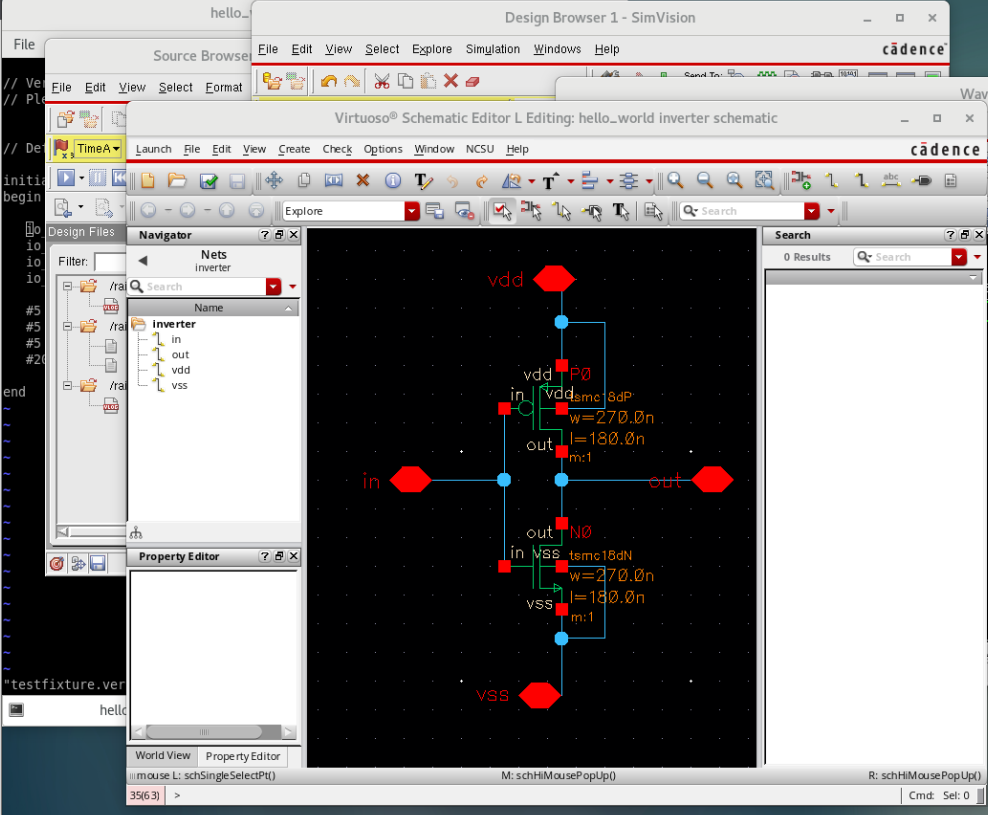
\includegraphics[width =\textwidth]{schematic.png}
	\label{schematic}
	\caption{Creating a cell}
\end{figure}

\begin{figure}[h]
	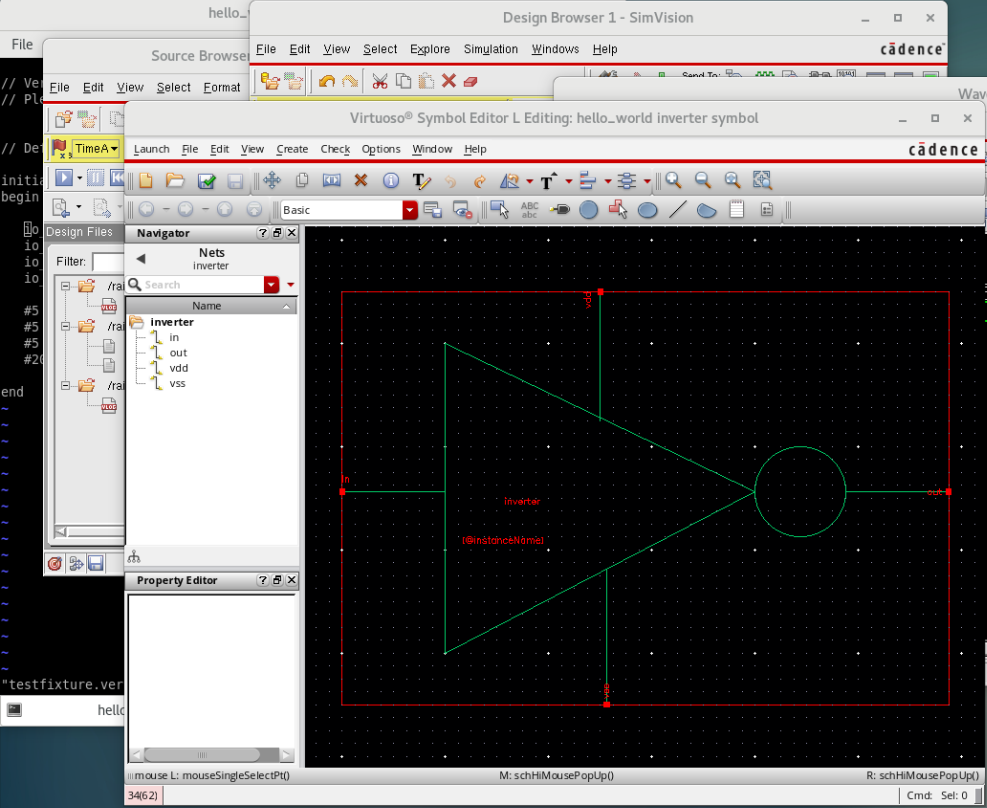
\includegraphics[width =\textwidth]{symbol.png}
	\label{symbol}
	\caption{Creating symbol}
\end{figure}

\begin{figure}[h]
	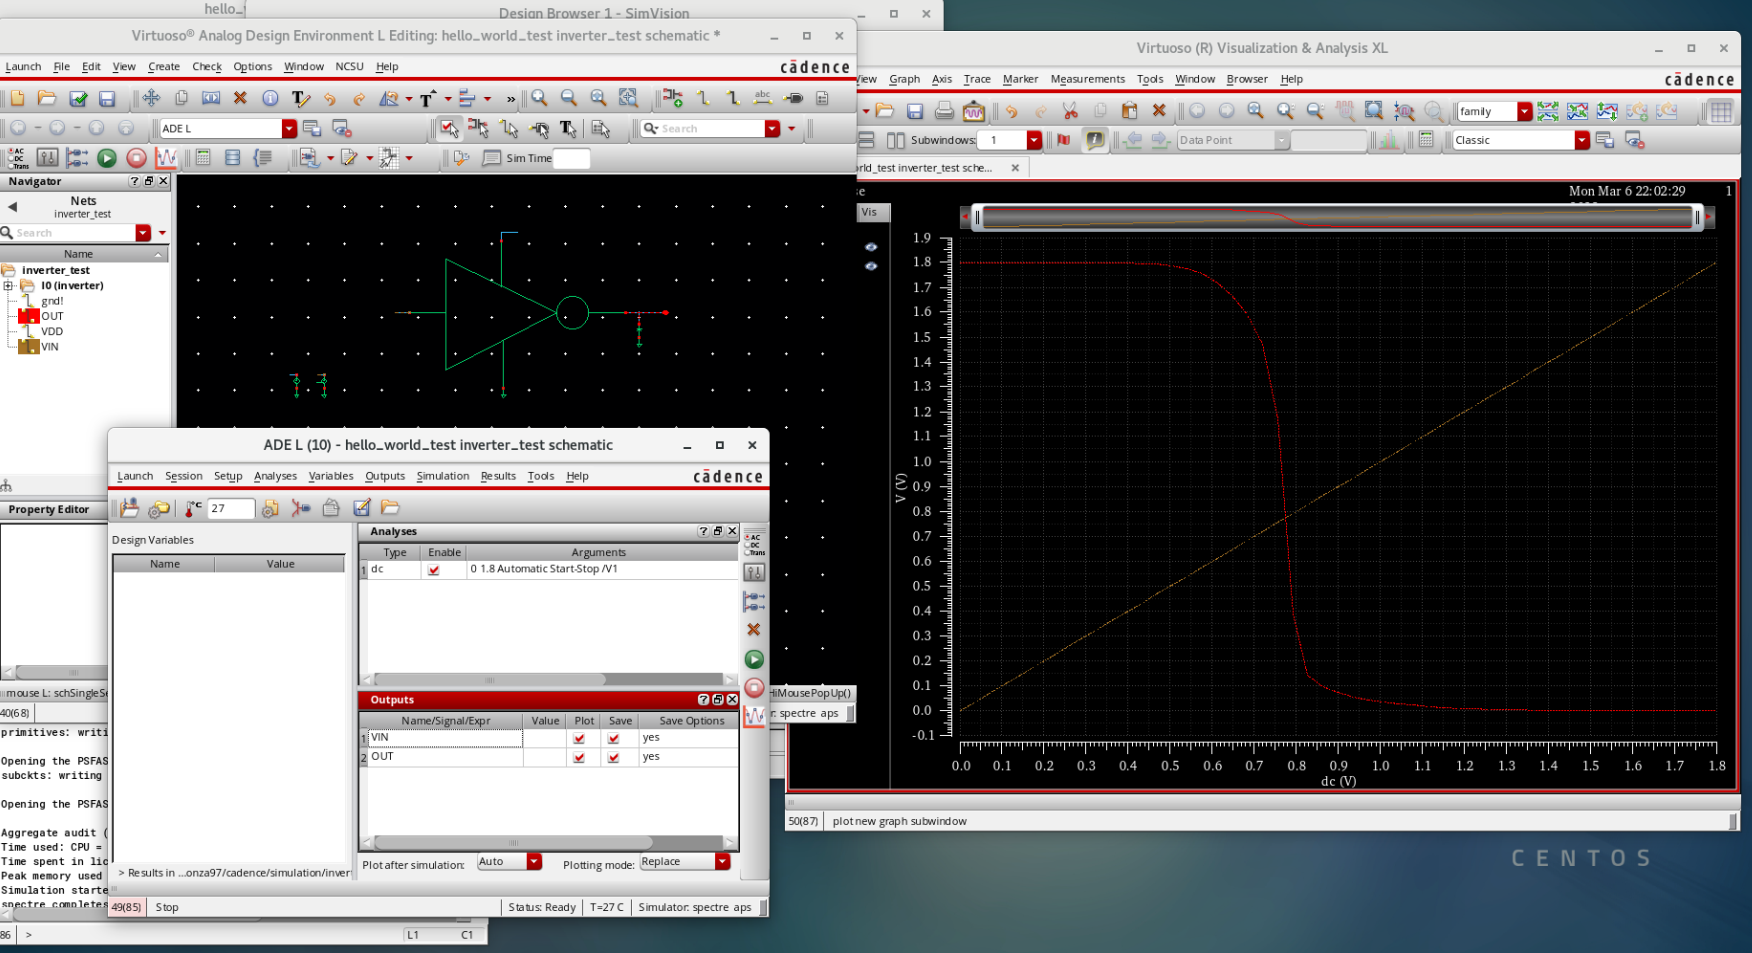
\includegraphics[width =\textwidth]{schemdcsweep.png}
	\label{schematicdcsweep}
	\caption{Schematic DC Sweep}
\end{figure}

\begin{figure}[h]
	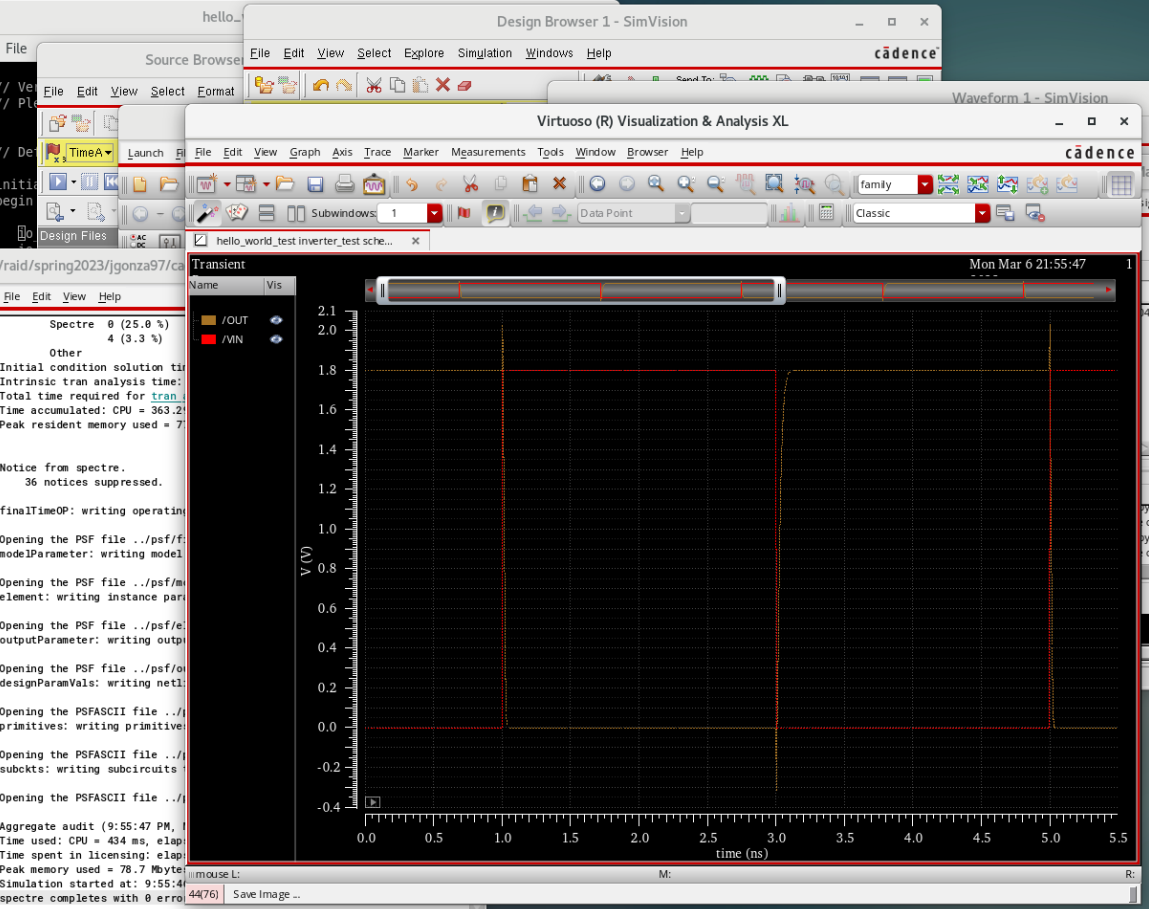
\includegraphics[width =\textwidth]{tran.png}
	\label{schematictrans}
	\caption{Transient Analysis}
\end{figure}

\begin{figure}[h]
	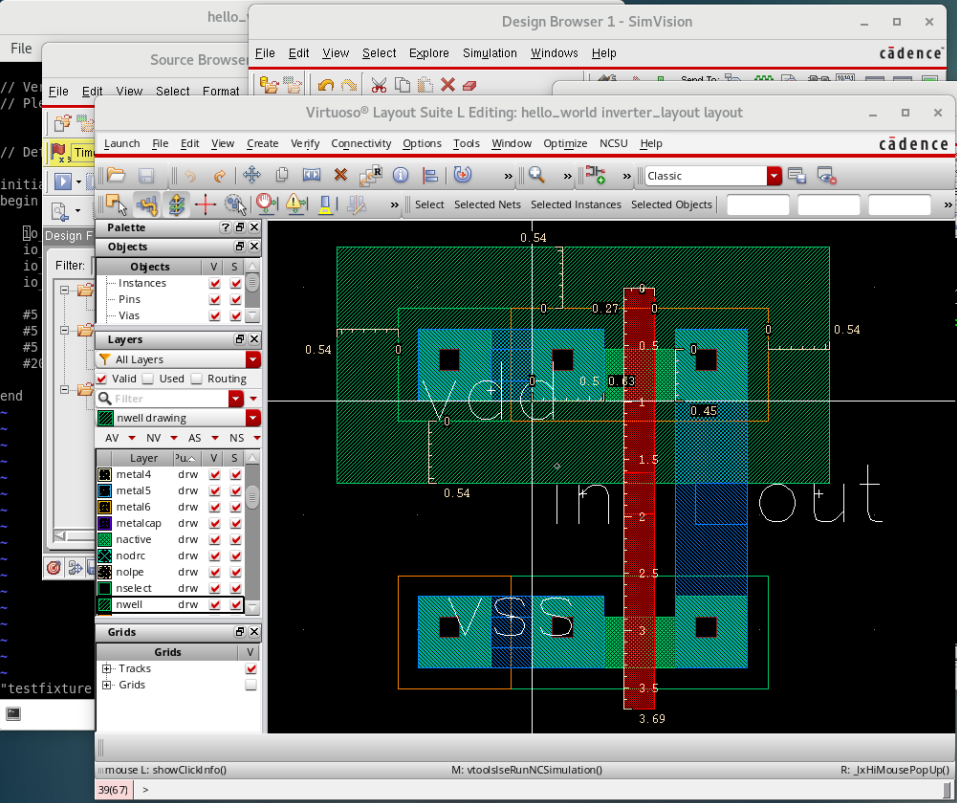
\includegraphics[width =\textwidth]{layout.png}
	\label{layout}
	\caption{Layout}
\end{figure}

\begin{figure}[h]
	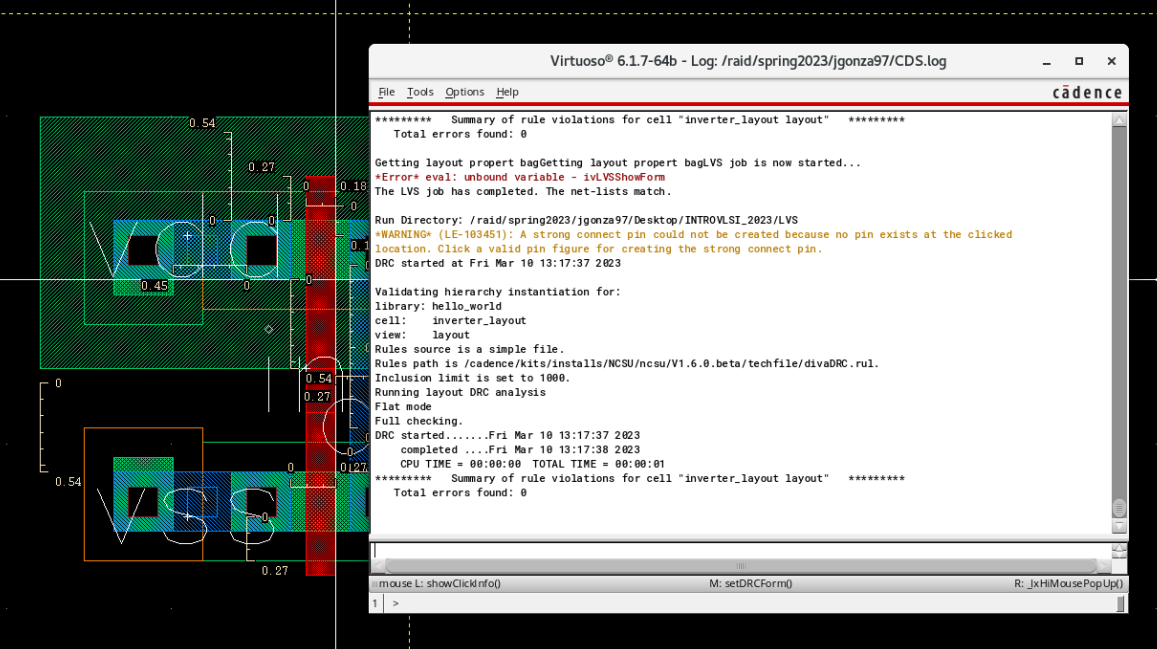
\includegraphics[width =\textwidth]{layoutDRC.png}
	\label{drc}
	\caption{Layout DRC Check}
\end{figure}

\begin{figure}[h]
	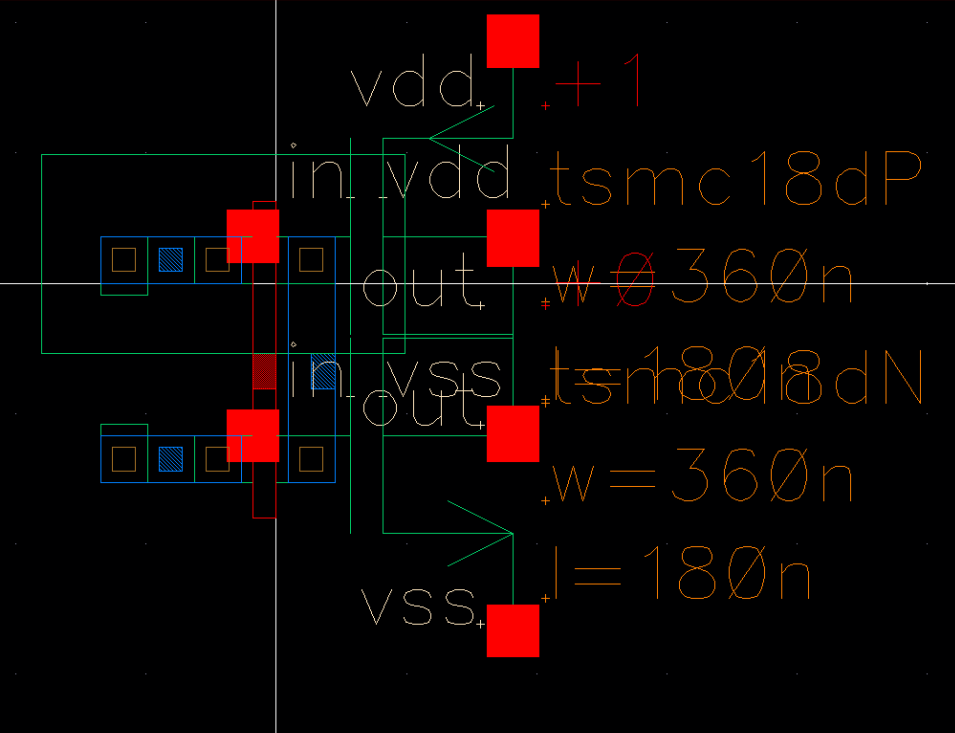
\includegraphics[width =\textwidth]{extracted.png}
	\label{extracted}
	\caption{Extracted}
\end{figure}

\begin{figure}[h]
	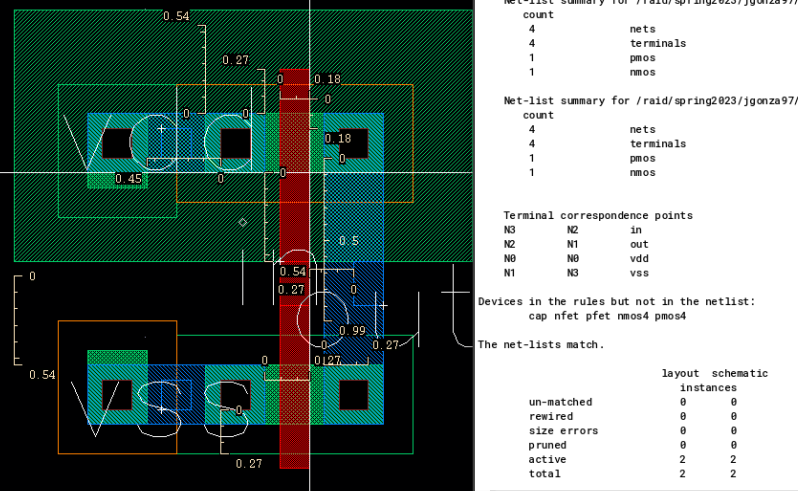
\includegraphics[width =\textwidth]{extractedLVS.png}
	\label{lvs}
	\caption{LVS Check}
\end{figure}


\begin{figure}[h]
	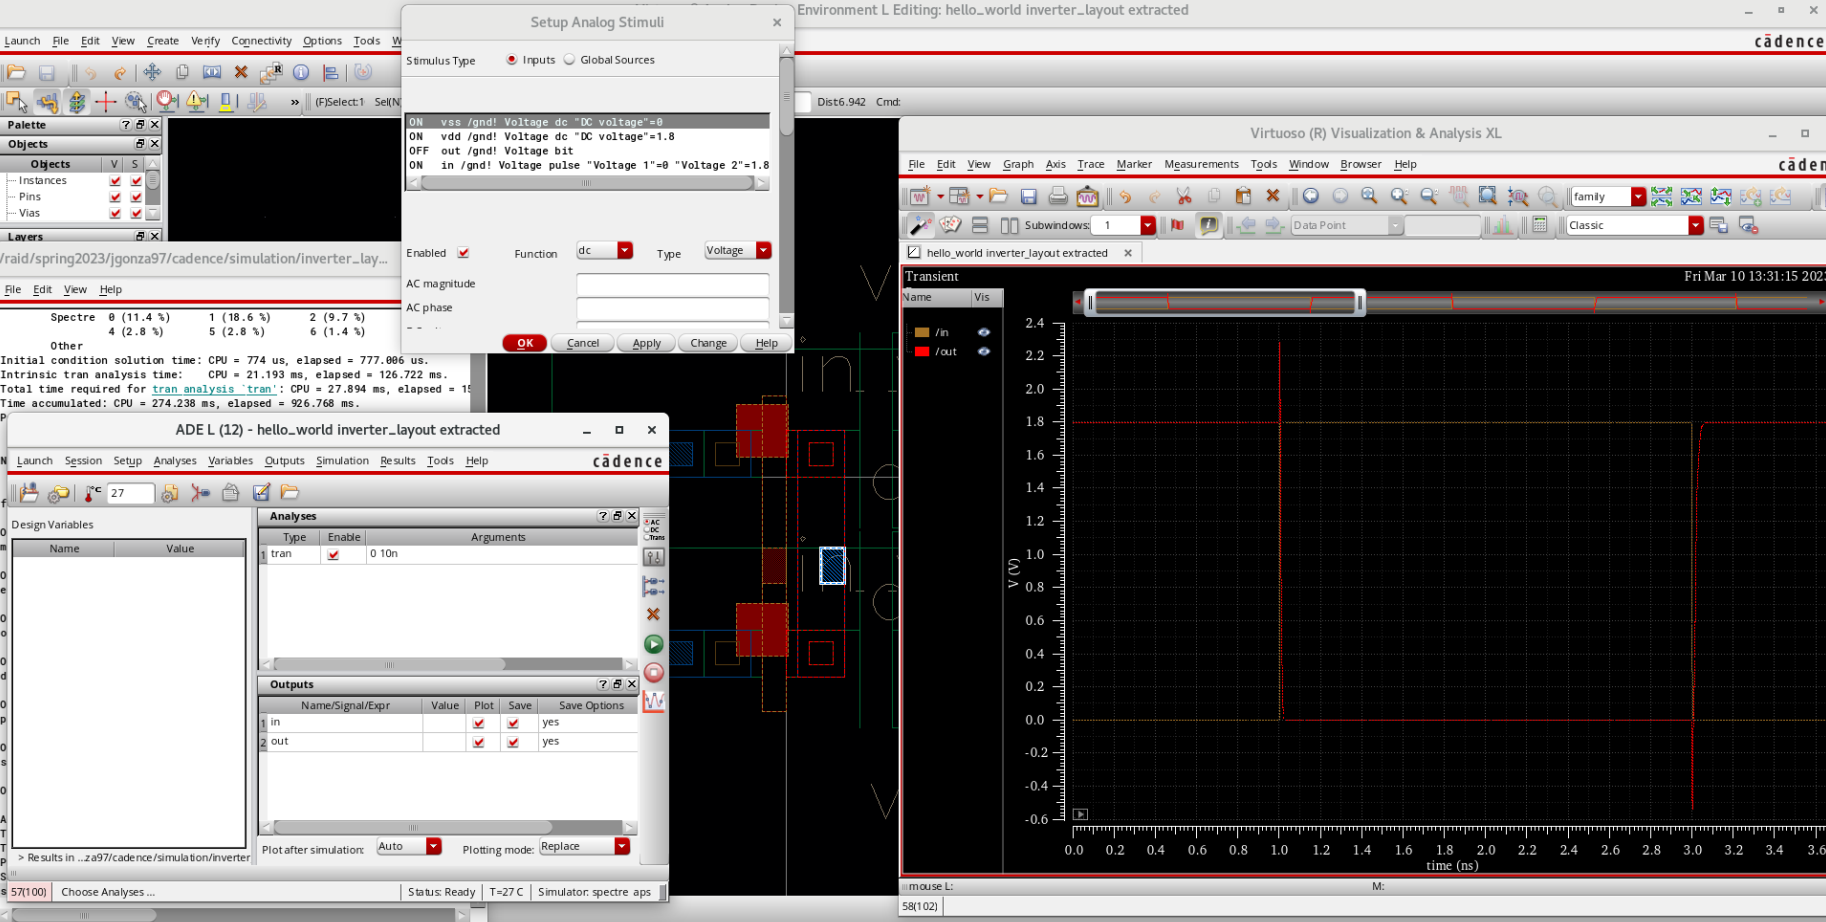
\includegraphics[width =\textwidth]{extractedtranstim.png}
	\label{extractedtrans}
	\caption{Extracted transient analysis}
\end{figure}

\begin{figure}[h]
	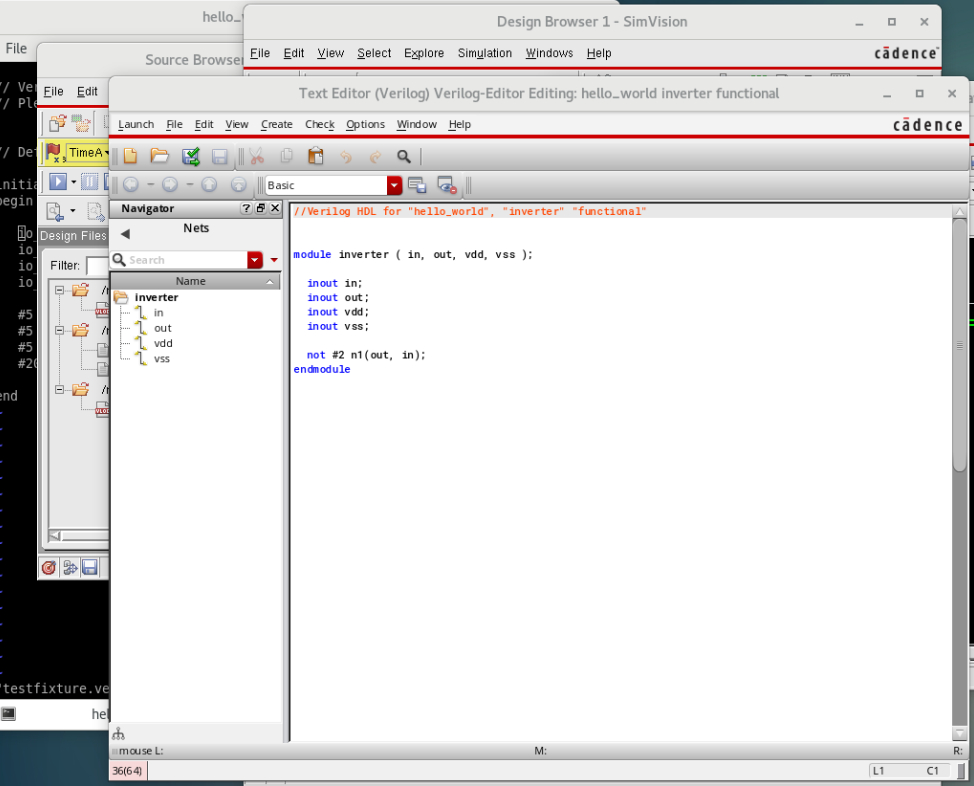
\includegraphics[width =\textwidth]{functional.png}
	\label{functional}
	\caption{Functional}
\end{figure}

\begin{figure}[h]
	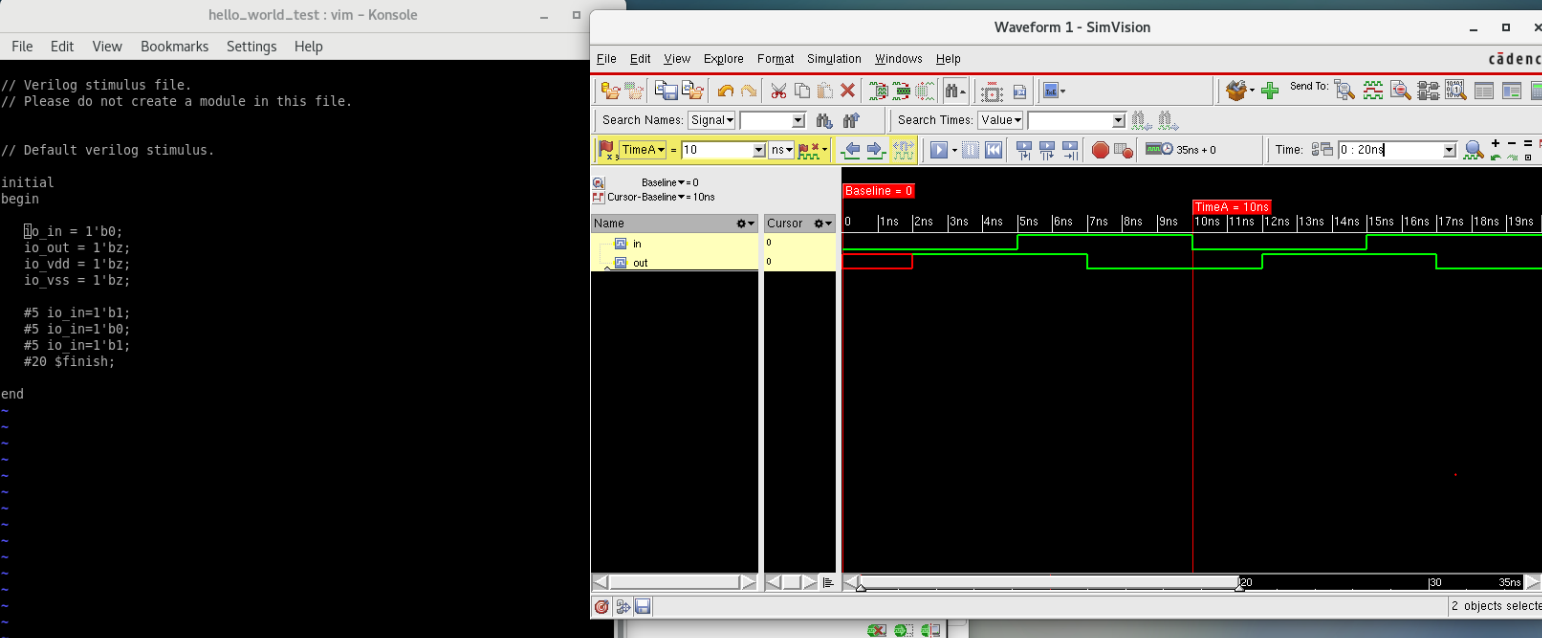
\includegraphics[width =\textwidth]{verilogoutput.png}
	\label{verilogoutput}
	\caption{Verilog .txt and Waveform output}
\end{figure}

\end{document}
